
%%%REFERENCIA EN CRIPT comienzo%%%%%%%%%%%%%%%%%%
%%No existen las hojas mencionadas%%%%

La Matem\'atica discreta es, simplemente, la parte de las Matem\'aticas que 
trata de objetos finitos, o en ocasiones  numerables. Decimos que esos objetos 
son discretos por oposici\'on a objetos {\itshape continuos} como los n\'umeros 
reales. 

As\'{\i}, por ejemplo, podemos decir que el estudio de los grupos finitos 
est\'a en la intersecci\'on del \'Algebra y la Matem\'atica discreta, o que el  
de los planos finitos lo est\'a  en la de la Geometr\'{\i}a y la Matem\'atica 
discreta.

Es claro que usando ordenadores \'unicamente podemos llegar a estudiar 
{\itshape objetos discretos}, finitos o numerables, y \'unicamente podemos 
aproximarnos a los objetos continuos mediante su {\itshape discretizaci\'on}, 
viendo, por ejemplo, un n\'umero real como un decimal con un n\'umero dado de 
cifras decimales.


En este cap\'{\i}tulo comenzamos con un resumen de la combinatoria b\'asica, 
que trata, esencialmente,  del siguiente problema:  suponemos dada
una familia de conjuntos finitos $X_{n,k}$, que depende de par\'ametros enteros,
en este caso $n$ y $k$. 

Se trata de encontrar f\'ormulas, que debemos determinar, 

\[\#(X_{n,k})=F(n,k)\]

\noindent que nos den el n\'umero de elementos de $X_{n,k}$ como una funci\'on
$F$ de los par\'ametros. Es decir, el problema central de la combinatoria
consiste en contar el n\'umero de elementos de conjuntos en funci\'on de
par\'ametros. 

Como no siempre se ha visto combinatoria en el Bachillerato, se puede consultar
un peque\~no resumen en 
\href{http://150.244.21.37/PDFs/MDISC/combinatoria.pdf}{este enlace.}  Cubre la parte m\'as
b\'asica, permutaciones, variaciones y combinaciones, junto con algunos
aspectos m\'as avanzados que ser\'an \'utiles al resolver los ejercicios de este
cap\'{\i}tulo.

En segundo lugar, se incluye una breve introducci\'on a la teor\'{\i}a de 
grafos, que son quiz\'a las estructuras finitas  con mayor n\'umero de 
aplicaciones a muy diversos problemas.

\section{Permutaciones, variaciones y combinaciones}

\begin{enumerate}
 \item {\sc Permutaciones:} Dado un conjunto $X$ con $n$ elementos, el conjunto
de todas las listas de longitud $n$ que podemos formar usando todos  los
elementos del conjunto  es el conjunto de {\itshape permutaciones} de $X$. 

En n\'umero de permutaciones de un conjunto de $n$ elementos es (?`por qu\'e?)
\[n!:=n\cdot (n-1)\cdot (n-2)\dots 3\cdot 2\cdot 1.\]

En {\sage} podemos generar el conjunto de permutaciones de 
$X:=\{1,2,\dots,n\}$ mediante \lstinline|p=Permutations(n)| y formar una lista
$L$ con todas las permutaciones usando \lstinline|L=p.list()|. 

\item{\sc Variaciones:}  Dado un conjunto $X$ con $n$ elementos, el conjunto
de todas las listas de longitud $k$ que podemos formar usando $k$   
elementos distintos del  conjunto  es el conjunto de {\itshape variaciones} de
$X$ usando $k$ elementos.

El n\'umero de variaciones de $X$ usando $k$ elementos es $n!/(n-k)!$  (?`por
qu\'e?).
 
 En {\sage} podemos generar el conjunto de variaciones  de 
$X:=\{1,2,\dots,n\}$ usando $k$ elementos  mediante
\lstinline|v=Permutations(n,k)| y formar una lista $L$ con
todas las variaciones usando \lstinline|L=v.list()|. 
 
 \item{\sc Combinaciones:}  Dado un conjunto $X$ con $n$ elementos, el conjunto
de todos los  subconjuntos  de longitud $k$ que podemos formar con elementos de
$X$  es el conjunto de {\itshape combinaciones} de $X$ usando $k$ elementos.
 
El n\'umero de combinaciones de $X$ usando $k$ elementos es
$\binom{n}{k}:=\frac{n!}{k!(n-k)!}$  (?`por
qu\'e?).
 
 En {\sage} podemos generar el conjunto de combinaciones   de 
$X:=\{1,2,\dots,n\}$ usando $k$ elementos  mediante \lstinline|c=Subsets(n,k)|
y formar una lista $L$ con todas los subconjuntos  usando
\lstinline|L=c.list()|.  Los elementos de esta lista son conjuntos no listas, y
si fuera necesario convertirlos podr\'{\i}amos usar 
\lstinline|[list(s) for s in L]|.


Sino especificamos un segundo argumento, \lstinline|c=Subsets(n)| se genera el
conjunto de todos los subconjuntos de $X$, es decir, {\itshape el conjunto de
partes de $X$} con n\'umero de elementos $2^n.$
 
 \end{enumerate}




\section{Funciones entre conjuntos finitos}

Una aplicaci\'on biyectiva, $f:A\longrightarrow B$, entre dos conjuntos, es una
aplicaci\'on al tiempo {\itshape inyectiva y sobreyectiva}. Una aplicaci\'on es
{\itshape inyectiva} si para cualesquiera dos elementos,  $a_1,a_2\in A$, tales
que  $f(a_1)=f(a_2)$ necesariamente $a_1=a_2$. Una aplicaci\'on es {\itshape
sobreyectiva} si para cualquier elemento $b\in B$ existe un elemento $a\in A$
tal que $f(a)=b$. 
 
Recordemos que:
\begin{enumerate}
\item Dadas funciones  $f:A\longrightarrow B$ y $g:B\longrightarrow C$ su
{\itshape composici\'on} $g\circ f:A  \longrightarrow C$ es la funci\'on
$g\circ f(a):=g(f(a)).$

Si dos aplicaciones biyectivas se pueden componer, la composici\'on es, de
nuevo, una biyecci\'on. 

\item En todo conjunto $A$ hay una biyecci\'on $1_A:A\longrightarrow A$ definida
mediante $1_A(a):=a$ para todo $a\in A.$

Toda biyecci\'on $f:A\longrightarrow B$ tiene una {\itshape inversa}
$g:B\longrightarrow A$, verificando $g\circ f=1_A$ y  $f\circ g=1_B$, que es
también una biyecci\'on.

\item Una funci\'on $f:A\longrightarrow B$ es inyectiva si y s\'olo si existe
una $g:B\longrightarrow A$ tal que $g\circ f=1_A$.

\item Una funci\'on $f:A\longrightarrow B$ es suprayectiva si y s\'olo si existe
una $g:B\longrightarrow A$ tal que $f\circ g=1_B$.
\end{enumerate}


En lo que sigue vamos a utilizar
ciertas estructuras de datos, listas y diccionarios, para representar
en el ordenador las funciones y poder trabajar con ellas. 

Para empezar puedes consultar la hoja
\href{http://sage.mat.uam.es:8888/home/pub/?/}{\tt
101-MDISC-biyecciones.sws}.

En estos ejercicios se entiende que {\itshape construir} un conjunto de funciones es definir
una funci\'on de {\sage} que devuelva, por ejemplo, una lista con elementos 
todas las funciones que se quiere construir. Construir estos conjuntos, que 
pueden ser enormes, permite atacar ciertos problemas mediante {\itshape fuerza 
bruta.} Como sabemos,  este m\'etodo de resolver problemas est\'a limitado por 
la cantidad de memoria RAM disponible y el tiempo que estemos dispuestos a 
esperar una soluci\'on.

Por otra parte, hemos visto que podemos usar como clave en un cierto sistema 
criptogr\'afico una biyecci\'on del alfabeto en s\'{\i} mismo, o, usando el 
\hyperref[oscurecer]{truco para oscurecer las frecuencias}, una biyecci\'on de 
un conjunto mucho mayor en s\'{\i} mismo. 
\par
\medskip
\par
\begin{ejer}
 Construye el conjunto $F(X,X)$ de todas las funciones de un conjunto finito
$X:=\{0,1,2,\dots,n-1\}$ en s\'{\i} mismo. Cada funci\'on debe venir dada
por un diccionario.
 \end{ejer}

\begin{ejer}
 Construye el subconjunto de las biyecciones de $X$ en $X$ y una
funci\'on de {\sage} que para cada biyecci\'on nos devuelva la
biyecci\'on inversa.
\end{ejer}

\begin{ejer}
 Dado dos conjuntos $X_n:=\{0,1,2,\dots,n-1\}$ e
$Y_m:=\{0,1,2,\dots,m-1\}$ con $m<n$ construye el conjunto $F(X_n,Y_m)$ de todas
las funciones de $X_n$ en $Y_m$.
\end{ejer}

\begin{ejer}
 Construye el subconjunto de todas las funciones suprayectivas de $X_n$ en
$Y_m$. ?`Cu\'antas hay?

Llamemos $Sup(n,m)$ al n\'umero de
funciones suprayectivas de $X_n$ en $Y_m$. Una f\'ormula que determine
$Sup(n,m)$ como una funci\'onn de $n$ y $m$ es bastante complicada, pero es
m\'as f\'acil obtener una f\'ormula recursiva que d\'e
$Sup(n+1,m)$ en funci\'on de $Sup(n,m)$ y $Sup(n,m-1)$. {\sc Deduce} esa
f\'ormula y {\sc compru\'ebala} con ayuda del programa realizado en
este apartado, es decir, programa la f\'ormula recursiva y comprueba que produce
los
mismos resultados que contar el n\'umero de funciones suprayectivas.
\end{ejer}

\begin{ejer}
  Dada una funci\'on suprayectiva $f:X \to Y$ construye el
conjunto de funciones de $g:Y \to X$ tales que $f\circ g=1_Y$.
\end{ejer}

\begin{ejer}
 Sea $\mathbb{Z}_m$ el conjunto de las clases de restos m\'odulo un
entero $m$, que representaremos como la lista \lstinline|srange(m)|.
Consideramos  la
funci\'on  $\Phi_k(n):\mathbb{Z}_m\to \mathbb{Z}_m$  definida
mediante $\Phi_k(n):=(k*n)\%m$. Queremos caracterizar los pares $(m,k)$ tales
que $\Phi_k$ es biyectiva. Si no conoces la respuesta debes experimentar con
distintos pares $(m,k)$ hasta entender lo que pasa, y si la conoces el ejercicio
consiste en producir c\'odigo para comprobarla.

{\sc Repite} el ejercicio, pero con la funci\'on
$\Psi_k(n):=(k^n)\%m$.
\end{ejer}

Puedes encontrar soluciones en la hoja
\href{http://sage.mat.uam.es:8888/home/pub/?/}{\tt
102-MDISC-funciones-sol.sws}.




\section{Acciones de grupos}
%%%POR QUE ESTA ESTO AQUI??????????????????????????????????%%%
Dados un grupo $G$ y un conjunto $X$, decimos que $G$ act\'ua en $X$ si hemos 
definido una funci\'on $\mu:G\times X\to X$ tal que $\mu(1,x)=x$, para todo 
$x\in X$, y $\mu(g_1,\mu(g_2,x))=\mu(g_1\cdot g_2,x).$


Habitualmente se denota la funci\'on $\mu$ mediante un producto, 
$\mu(g,x)=:g\cdot x$ que hay que distinguir cuidadosamente del producto en el 
grupo $G$. La primera propiedad en la definici\'on de una acci\'on de un grupo 
en un conjunto puede enunciarse diciendo que el elemento neutro en el grupo, 
$1\in G$ es {\itshape neutro para la acci\'on}, y la segunda es una {\itshape 
propiedad asociativa.}

El {\itshape conjunto de \'orbitas} $X/G$ para una acci\'on de $G$ en $X$ es el 
conjunto cociente $X$ para la relaci\'on de equivalencia  
\begin{center}
{\itshape $x_1\sim x_2$ si y s\'olo si existe $g\in G$ tal que $x_2=g\cdot 
x_1.$}
\end{center}

Cada clase de equivalencia,$[x]$,  es la \'orbita $o(x)$ de uno cualquiera de 
sus elementos $x$, es decir,
\[[x]=o(x)=\{g\cdot x\mid g\in G\}.\]

Estas nociones, {\itshape acci\'on de un grupo en un conjunto y conjunto de 
\'orbitas}, son importantes en geometr\'{\i}a con $X$ un conjunto de figuras
geom\'etricas, por ejemplo tri\'angulos o c\'onicas planas, y $G$ un grupo, por 
ejemplo el grupo de transformaciones afines del plano, que utilizamos para 
clasificar las figuras.

As\'{\i}, todos los tri\'angulos son equivalentes 
respecto al grupo af\'{\i}n y tenemos una \'unica \'orbita, pero no todas las 
c\'onicas son equivalentes respecto al mismo grupo: podemos transformar una 
circunferencia en una elipse pero no una circunferencia en una par\'abola.  

\hyperref[orbitas]{{\sc Hemos usado} la palabra {\itshape \'orbita}} para referirnos al conjunto de los 
iterados de un elemento $x\in X$ mediante una funci\'on $f:X\to X$:
\[o(x):=\{x,f(x),f^2(x):=f(f(x)),f^3(x):=f(f(f(x))),\dots\},\]
\noindent y la relaci\'on con una \'orbita de una acci\'on de un grupo debe ser 
clara: {\itshape si $f$ es biyectiva} forma junto con todos sus iterados, con 
exponente positivo o negativo, un grupo 
\[G:=\{\dots,f^{-2},f^{-1},f^{0}=identidad,f,f^2,f^3,\dots \},\]
\noindent y la \'orbita de $x$ para este  grupo es la uni\'on de la \'orbita de 
$x$ para $f$ con la \'orbita de $x$ para la funci\'on inversa $f^{-1}$.


\section{Grafos}
Los grafos son objetos geom\'etricos $1$-dimensionales:


{\itshape Un grafo $G=(V,E)$ dirigido con conjunto de v\'ertices $V$ finito es 
un subconjunto $E\subset 
V\times V$.  }



Entonces, un grafo puede verse como un conjunto de {\itshape v\'ertices} $V$ 
junto con un conjunto de pares ordenados de v\'ertices, que representamos como 
flechas 
que unen el primer v\'ertice  del par con el segundo, con la flecha apuntando 
al segundo, y llamamos {\itshape ejes} del grafo. Podemos 
entonces representar el grafo mediante un dibujo, por ejemplo en el plano, y 
verlo como un objeto geom\'etrico $1$-dimensional. 

{\itshape Un grafo con conjunto de v\'ertices $V$ finito es un subconjunto 
$E\subset V\times V/\mathbb{Z}_2$, con $V\times V/\mathbb{Z}_2$ el conjunto 
\'orbitas para la acci\'on de $\mathbb{Z}_2:=\{1,\sigma\}$ en $V\times V$ 
definida por $\sigma(v_1,v_2):=(v_2,v_1).$}

En el caso de un grafo, no dirigidos, representamos los ejes como segmentos sin 
la flecha, y cuando queramos indicar que un grafo est\'a dirigido lo 
indicaremos expl\'{\i}citamente. 

{\sc Algunas definiciones:}
\begin{enumerate}
 \item Un eje que une un v\'ertice consigo mismo se dice que es un {\itshape 
lazo.}
 
 \item Un {\itshape camino} en el grafo desde el v\'ertice $v$ al $v^{\prime}$ 
es una sucesi\'on de ejes $e_1,e_2,\dots,e_n$ tales que $e_1$ contiene a $v$, 
$e_n$ a $v^{\prime}$ y el eje $e_i$ tiene un v\'ertice com\'un con $e_{i+1}$ 
para $1\le i<n$. 

Si el grafo est\'a dirigido necesitamos adem\'as que las flechas apunten todas 
de $v$ a $v^{\prime}.$

\item Un {\itshape ciclo} en el grafo es un camino cerrado, es decir,  tal que 
$v$ coincide con $v^{\prime}.$

\item Un {\itshape \'arbol} es un grafo sin ciclos. 

\item Un grafo es {\itshape conexo} si para cada par de v\'ertices existe un 
camino que los une. Un grafo no conexo es una {\itshape uni\'on disjunta} de 
grafos,  que llamamos las {\itshape componentes}, de forma que no hay ejes 
entre una componente y otra distinta. 
 
 \item Un grafo se dice que es {\itshape planar} si puede ser representado en 
el plano sin que se corten sus ejes. 
 
 \item Un grafo es {\itshape euleriano} si existe un ciclo que pasa una \'unica 
vez por cada eje.
 
 \item Un grafo es {\itshape hamiltoniano} si existe un ciclo que contiene una 
\'unica vez cada v\'ertice. 
 
 \item Denotamos los v\'ertices de un grafo como $V:=\{v_1,v_2,\dots,v_n\}$. La 
{\itshape matriz de adyacencia} del grafo es la matriz $M$  $n\times n$ con 
entradas ceros y unos definida mediante 
\[M_{ij}=
 \begin{cases}
  1 \text{ si hay un eje que una $v_i$ con $v_j$}\\
  0 \text{ si no lo hay}
 \end{cases}
\]
 La matriz de adyacencia contiene toda la informaci\'on sobre el grafo, y 
mediante el producto de matrices permite extraer nueva informaci\'on.La matriz 
de un grafo no dirigido es sim\'etrica.
 
 \item Dos grafos son {\itshape isomorfos} si existe una biyecci\'on entre sus 
conjuntos de v\'ertices de forma que dos ejes est\'an unidos mediante un eje en 
el primer grafo si y s\'olo si sus im\'agenes est\'an unidas mediante un eje en 
el segundo.


Es decir, dos grafos son isomorfos si son el mismo salvo las etiquetas de los 
v\'ertices. 

\item Llamamos {\itshape grado de un v\'ertice} al n\'umero de ejes que 
contienen al v\'ertice. 

\item Un grafo se dice {\itshape regular} si todos los v\'ertices tienen el 
mismo grado. 

\item El {\itshape grafo completo} con $n$ v\'ertices es el que tiene todos los 
ejes posibles, es decir, su conjunto de ejes ed $V\times V.$

\end{enumerate}

\begin{ejer}
 Sea $G$ un grafo, dirigido o no, con matriz de adyacencia $M$. 
 \begin{enumerate}
  \item Demuestra que la entrada $(M^n)_{ij}$ es un entero que cuenta el 
n\'umero de caminos con $n$ ejes, dirigidos si el grafo es dirigido, desde el 
v\'ertice $v_i$ 
al v\'ertice $v_j$.

\item Demuestra que el n\'umero de tri\'angulos, ciclo con tres ejes,  
contenidos en el grafo  es 
   un sexto de la traza de $M^3$.
  
 \end{enumerate}
 \end{ejer}



\subsection{Grafos en {\sage}}

\begin{enumerate}
 \item {\sc Construcci\'on  de grafos:}
 \begin{enumerate}
 \item {\sage} conoce una gran cantidad de grafos que tienen nombre. Se puede 
ver la lista escribiendo en una celda \lstinline|graphs.| y pulsando la tecla 
del tabulador. Por ejemplo, 
 \begin{lstlisting}
  G = graphs.DurerGraph()
  show(G)
 \end{lstlisting}
\noindent produce este grafo:
\begin{center}
 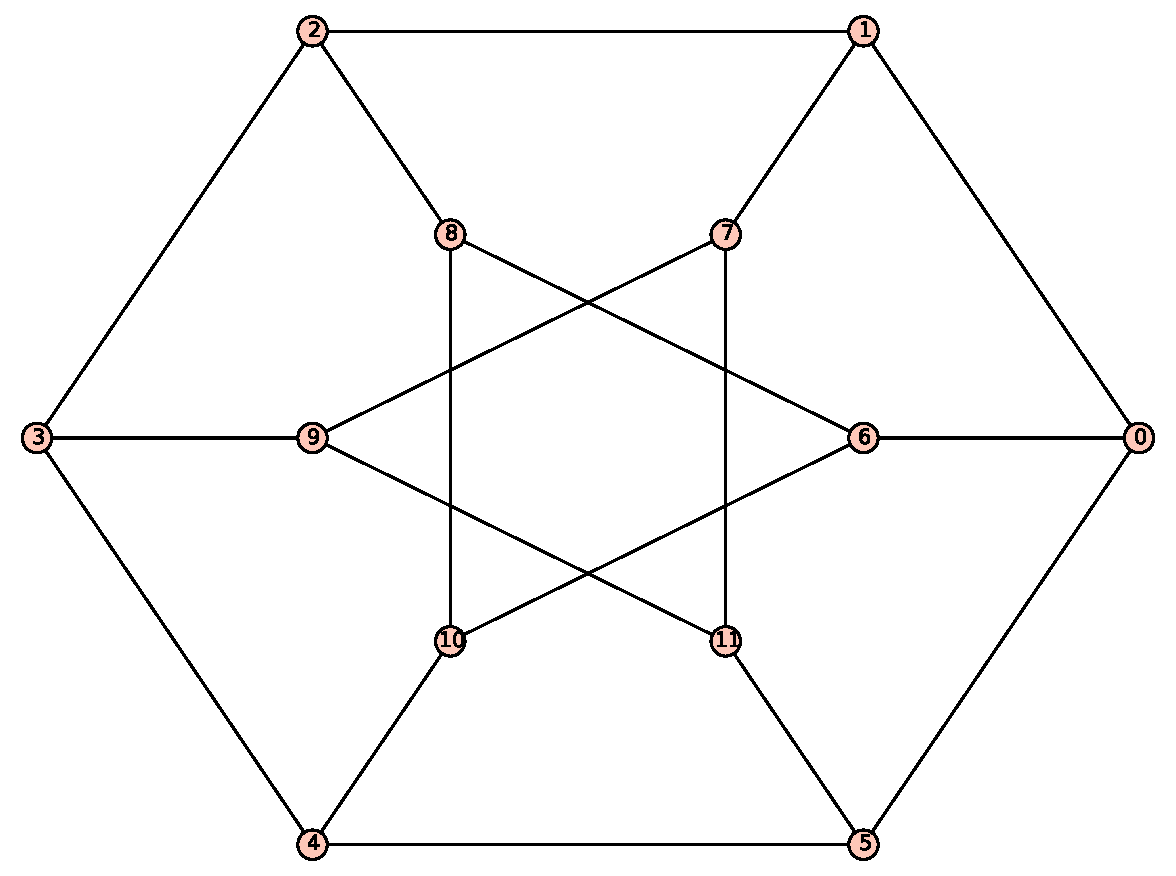
\includegraphics[scale=0.3]{durero}
\end{center}
%%\item 
 %%\end{enumerate}
\item La instrucci\'on 
\begin{lstinline}
 G1 = graphs.RandomGNP(n,p)
\end{lstinline}
\noindent produce un grafo aleatoriamente construido con $n$ v\'ertices y 
probabilidad $p$ de incluir cada uno de los posibles ejes. Cuando $p$ es baja 
obtendremos casi siempre un grafo no conexo mientras que cuando es alta ser\'a 
casi seguramente conexo.

\item La instrucci\'on 
\begin{lstlisting}
 G2 = graphs.RandomGNM(n,m)
\end{lstlisting}
\noindent produce un grafo aleatoriamente elegido con $n$ v\'ertices y 
$m$ ejes. Elegimos el grafo, de entre todos los grafos con $n$ v\'ertices y $m$ 
ejes, de manera equiprobable.

\item Podemos generar un grafo usando su matriz de adyacencia:
\begin{lstlisting}
M1 = matrix(ZZ,7,[randint(0,1) for muda in srange(49)])
M = (M1+M1.transpose())/2
G3 = Graph(M)
show(G3)
\end{lstlisting}

Como se trata de un grafo no dirigido, su matriz debe ser sim\'etrica y 
simetrizamos la matriz $M1$, que ha sido generada aleatoriamente,  en la 
segunda l\'{\i}nea. 

\item Tambi\'en podemos dar expl\'{\i}citamente la lista de ejes:
\begin{lstlisting}
G4=Graph(7)                #7 vertices
ejes=[(1,3),(2,5)]         #Una lista de pares (duplas) de vertices 
G4.add_edges(ejes)
show(G4)
\end{lstlisting}
%%\end{enumerate}
\end{enumerate}
\item {\sc M\'etodos para grafos:}

\begin{enumerate}
 \item Como en general con {\sage}, podemos ver todos los m\'etodos que se 
aplican a los grafos creando un grafo, por ejemplo con nombre $G$, y pulsando 
el tabulador en una celda en la que hemos escrito \lstinline|G.|. La cantidad 
de m\'etodos existentes es enorme, y en este curso s\'olo llegaremos a usar 
unos pocos. 
 
 \item Disponemos de m\'etodos, con respuesta booleana, para comprobar si un 
grafo verifica una cierta propiedad. Son los m\'etodos del tipo 
\lstinline|G.is_...|, como por ejemplo
\begin{enumerate}
\item \lstinline|G.is_connected()|.
\item \lstinline|G.is_eulerian()|.
\item \lstinline|G.is_hamiltonian()|.
\item \lstinline|G.is_planar()|.
\item \lstinline|G.is_tree()|.
\item \lstinline|G.is_regular()|.
\item \lstinline|G1.is_isomorphic(G2)|.
\end{enumerate}

Si el grafo $G$ resulta ser euleriano, podr\'{\i}amos ver un ciclo euleriano 
mediante \lstinline|show(G.eulerian_circuit())|, y en el caso hamiltoniano 
mediante \lstinline|show(G2.hamiltonian_cycle())|.

\item Podemos obtener la matriz de adyacencia de un grafo $G$ mediante 
\lstinline|M=G.adjacency()|, de forma  que, despu\'es de ejecutar esa 
instrucci\'on,  podemos operar con la matriz $M$.
 
\end{enumerate}
\end{enumerate}

\begin{ejem}
 Encontrar el mayor subconjunto de enteros entre $1$ y $100$ con la propiedad 
de que no hay dos de ellos cuya diferencia sea, en valor absoluto, un cuadrado. 
 
 
 Se puede resolver mediante este c\'odigo
 
 
 \begin{lstlisting}
n=100
G=Graph(n)
cuadrados=[i*i for i in srange(sqrt(n))]
ejes=[(i,j) for (i,j) in CartesianProduct(srange(n),srange(n)) if (i!=j and 
abs(i-j) in cuadrados)]
G.add_edges(ejes)
L = G.independent_set();L
 \end{lstlisting}
 
 \noindent teniendo en cuenta que \lstinline|G.independent_set()| devuelve un 
conjunto maximal de v\'ertices, i.e. no podemos a\~nadir ning\'un v\'ertice sin que deje de 
tener la propiedad que enunciamos a continuaci\'on,   tal que no hay ejes entre ning\'un par de v\'ertices del 
subconjunto. 

\end{ejem}
%\end{enumerate}